% !TeX program = pdfLaTeX
\documentclass[12pt]{article}
\usepackage{amsmath}
\usepackage{graphicx,psfrag,epsf}
\usepackage{enumerate}
\usepackage{natbib}
\usepackage{textcomp}
\usepackage[hyphens]{url} % not crucial - just used below for the URL
\usepackage{hyperref}
\providecommand{\tightlist}{%
  \setlength{\itemsep}{0pt}\setlength{\parskip}{0pt}}

%\pdfminorversion=4
% NOTE: To produce blinded version, replace "0" with "1" below.
\newcommand{\blind}{0}

% DON'T change margins - should be 1 inch all around.
\addtolength{\oddsidemargin}{-.5in}%
\addtolength{\evensidemargin}{-.5in}%
\addtolength{\textwidth}{1in}%
\addtolength{\textheight}{1.3in}%
\addtolength{\topmargin}{-.8in}%

%% load any required packages here



% Pandoc citation processing

\usepackage{float}
\usepackage{mathtools}
\usepackage{natbib}
\usepackage[linesnumbered,ruled,vlined]{algorithm2e}
\setcitestyle{numbers,square,comma}
\usepackage{verbatim}
\usepackage{amsthm}
\usepackage{comment}

\begin{document}


\def\spacingset#1{\renewcommand{\baselinestretch}%
{#1}\small\normalsize} \spacingset{1}


%%%%%%%%%%%%%%%%%%%%%%%%%%%%%%%%%%%%%%%%%%%%%%%%%%%%%%%%%%%%%%%%%%%%%%%%%%%%%%

\if0\blind
{
  \title{\bf Manifold Clustering for Latent Structure Block Models}

  \author{
        John Koo \\
    Department of YYY, University of XXX\\
      }
  \maketitle
} \fi

\if1\blind
{
  \bigskip
  \bigskip
  \bigskip
  \begin{center}
    {\LARGE\bf Manifold Clustering for Latent Structure Block Models}
  \end{center}
  \medskip
} \fi

\bigskip
\begin{abstract}
The text of your abstract. 200 or fewer words.
\end{abstract}

\noindent%
{\it Keywords:} block models, community detection, coordinate descent,
latent structure models, manifold clustering, random dot product graph
\vfill

\newpage
\spacingset{1.45} % DON'T change the spacing!

\newcommand{\diag}{\mathrm{diag}}
\newcommand{\tr}{\mathrm{Tr}}
\newcommand{\blockdiag}{\mathrm{blockdiag}}
\newcommand{\indep}{\stackrel{\mathrm{ind}}{\sim}}
\newcommand{\iid}{\stackrel{\mathrm{iid}}{\sim}}
\newcommand{\Bernoulli}{\mathrm{Bernoulli}}
\newcommand{\Betadist}{\mathrm{Beta}}
\newcommand{\BG}{\mathrm{BernoulliGraph}}
\newcommand{\Uniform}{\mathrm{Uniform}}
\newcommand{\PABM}{\mathrm{PABM}}
\newcommand{\RDPG}{\mathrm{RDPG}}
\newcommand{\GRDPG}{\mathrm{GRDPG}}
\newcommand{\Multinomial}{\mathrm{Multinomial}}
\newtheorem{theorem}{Theorem}
\newtheorem{lemma}{Lemma}
\newtheorem{proposition}{Proposition}
\theoremstyle{remark}
\newtheorem{remark}{Remark}
\theoremstyle{definition}
\newtheorem{definition}{Definition}
\newtheorem{example}{Example}
\newcommand{\dd}{\mathrm{d}}
\newcommand{\as}{\stackrel{\mathrm{a.s.}}{\to}}

\hypertarget{introduction}{%
\section{Introduction}\label{introduction}}

\hypertarget{latent-structure-block-models}{%
\section{Latent Structure Block
Models}\label{latent-structure-block-models}}

All block models are latent structure block models.

\hypertarget{methods}{%
\section{Methods}\label{methods}}

Here, we provide two algorithms for LSBM community detection.

\hypertarget{nonintersecting-manifolds}{%
\subsection{Nonintersecting Manifolds}\label{nonintersecting-manifolds}}

\hypertarget{preliminary-theory}{%
\subsubsection{Preliminary Theory}\label{preliminary-theory}}

\hypertarget{distributions-of-differences-of-order-statistics}{%
\paragraph{Distributions of differences of order
statistics}\label{distributions-of-differences-of-order-statistics}}

Let \(D_i = X_{(i+1)} - X_{(i)}\). Then if \(\max_i D_i < \delta\), we
have sufficient separation of points in \(\mathcal{M}_1\). Then it is
sufficient to quantify \(P(\max_i D_i > \delta)\) as a function of \(n\)
and \(\delta\) and show that this converges to zero as \(n\) grows to
\(\infty\).

We denote \(f(x)\) as the density of each \(X_i\), \(g_i(x)\) as the
density of \(X_{(i)}\), \(g_{ij}(x, y)\) as the joint density of
\(X_{(i)}, X_{(j)}\), and \(h_i(d)\) as the density of \(D_i\) (with
corresponding capital letters for the cumulative distribution
functions).

The following are taken as given\footnote{\url{https://en.wikipedia.org/wiki/Order_statistic}}:

\begin{enumerate}
\def\labelenumi{\arabic{enumi}.}
\tightlist
\item
  \(g_i(x) = \frac{n!}{(n-i)! (i-1)!} (F(x))^{i-1} (1 - F(x))^{n-i} f(x)\).
\item
  \(g_{ij}(x, y) = \frac{n!}{(i-1)! (j-i-1)! (n-j)!} (F(x))^{i-1} (F(y) - F(x))^{j-i-1} (1 - F(y))^{n-j} f(x) f(y)\).
\item
  By convolution,
  \(h_i(d) = \int_0^{1} g_{i, i+1} (x, x + d) \mathrm{d}x\).
\end{enumerate}

\begin{lemma}[The probability density function of $D_i$]
\begin{equation}
\label{eq:pdf}
h_i(d) = \int_0^{1-d} \frac{n!}{(i-1)! (n-i-1)!} (F(x))^{i-1} (1 - F(x+d))^{n-i-1} f(x) f(x+d) \mathrm{d}x 
\end{equation}
\end{lemma}

\begin{proof}
This is just a direct consequence of 2 and 3 under the given statements. 
We also note that because the support of $X_i$ is $[0, 1]$, 
the integral only needs to be evaluated from $0$ to $1 - d$ 
because of the $f(x+d)$ and $1 - F(x+d)$ terms.
\end{proof}

\begin{lemma}[The cumulative distribution function of $D_i$]

\begin{equation}
\label{eq:cdf}
P(D_i < \delta) = H_i(\delta) = 1 - \int_0^{1-\delta} \frac{n!}{(n-i)! (i-1)!} (F(x))^{i-1} (1 - F(x + \delta))^{n-i} f(x) \mathrm{d}x
\end{equation}
\end{lemma}

\begin{proof}
$$
\begin{aligned}
H_i(\delta) & = \int_x^{x+\delta} h_i(d) \mathrm{d}d \\
& = \int_x^{x+\delta} \int_0^{1} \frac{n!}{(i-1)! (n-i-1)!} ((F(x))^{i-1} (1 - F(x+d))^{n-i-1} f(x) f(x+d) \mathrm{d}x \mathrm{d}d \\
& = \int_0^{1} \frac{n!}{(i-1)! (n-i-1)!} (F(x))^{i-1} f(x) \int_x^{x+\delta} (1 - F(x+d))^{n-i-1} f(x+d) \mathrm{d}d \mathrm{d}x \\
& = \int_0^{1} \frac{n!}{(i-1)! (n-i-1)!} (F(x))^{i-1} f(x) \int_{F(x)}^{F(x+\delta)} (1 - u)^{n-i-1} \mathrm{d}u \mathrm{d}x \\
& = \int_0^{1} \frac{n!}{(i-1)! (n-i)!} (F(x))^{i-1} f(x) ((1 - F(x))^{n-i} - (1 - F(x + \delta))^{n-i}) \mathrm{d}x \\ 
& = \int_0^1 g_i(x) \mathrm{d}x - \int_0^1 \frac{n!}{(i-1)! (n-i)!} (F(x))^{i-1} (1 - F(x + \delta))^{n-i} f(x) \mathrm{d}x \\
& = 1 - \int_0^1 \frac{n!}{(i-1)! (n-i)!} (F(x))^{i-1} (1 - F(x + \delta))^{n-i} f(x) \mathrm{d}x \\
\end{aligned}
$$

Because of the $x + \delta$ term, we can't actually evaluate this integral all the way up to $1$, and so we are left with 
$$
\begin{aligned}
& = 1 - \int_0^{1 - \delta} \frac{n!}{(i-1)! (n-i)!} (F(x))^{i-1} (1 - F(x + \delta))^{n-i} f(x) \mathrm{d}x.
\end{aligned}
$$
\end{proof}

\hypertarget{uniform-case}{%
\paragraph{Uniform case}\label{uniform-case}}

\begin{lemma}[Differences between order statistics of a uniform distribution]
If $X_1, ..., X_n \stackrel{\mathrm{iid}}{\sim}\mathrm{Uniform}(0, 1)$, then each $D_i \sim \mathrm{Beta}(1, n)$.
\end{lemma}

\begin{proof}
We begin with Eq. (\ref{eq:pdf}), plugging in $f(x) = 1$ and $F(x) = x$:

$$
h_i(d) = \int_0^{1-d} \frac{n!}{(i-1)! (n-i-1)!} x^{i-1} (1-x-d)^{n-i-1} \mathrm{d}x
$$

Then we proceed with integration by parts, setting 
$u = x^{i-1} \implies du = (i-1) x^{i-2}$ and 
$dv = (1-x-d)^{n-i-1} dx \implies v = -\frac{1}{n-i} (1-x-d)^{n-i-1}$. 
Note that $u v |_0^{1-d} = 0$ in this case. This yields

$$
= \frac{n!}{(i-1)! (n-i-1)!} \int \frac{i-1}{n-i} x^{i-2} (1-x-d)^{n-i} \mathrm{d}x
$$

Then applying integration by parts again until the $x^p$ term disappears, we get:

$$
\begin{aligned}
& = \frac{n!}{(i-1)! (n-i-1)!} \frac{(i-1)!}{(n-i) \cdots (n-2)} \int_0^{1-d} (1-x-d)^{n-2} \mathrm{d}x \\
& = -\frac{n (n-1)}{n-1} (1-x-d)^{n-1} \Big|_0^{1-d} \\
& = n (1 - d)^{n-1}
\end{aligned}
$$

This the density function for $\mathrm{Beta}(1, n)$, completing the proof.
\end{proof}

\begin{theorem}
Let $X_1, ..., X_n \stackrel{\mathrm{iid}}{\sim}\mathrm{Uniform}(0, 1)$. 
Then for any $\epsilon$ and $\delta > 0$, 
there exists an $N = O \big(\frac{-\log \epsilon}{\delta} \big)$ such that 
$P(\max_i X_{(i+1)} - X_{(i)} < \delta) \geq 1 - \epsilon$ when $n > N$.
\end{theorem}

\begin{proof}[Proof (sketch)]
Since $X_{(i+1)} - X_{(i)} = D_i \sim \mathrm{Beta}(1, n)$, 
$P(X_{(i+1)} - X_{(i)} < \delta) = 1 - (1 - \delta)^n $. This yields

$$
\begin{aligned}
P(\max_i D_i < \delta) & \geq (P(D_i < \delta))^{n-1} \\
& = (1 - (1 - \delta)^n)^{n-1} \\
& \approx e^{-n \exp(-n \delta)}.
\end{aligned}
$$

In the limit $n \to \infty$, this goes to 1.
\end{proof}

\hypertarget{general-case-for-one-dimensional-manifolds}{%
\paragraph{General case for one-dimensional
manifolds}\label{general-case-for-one-dimensional-manifolds}}

\begin{theorem}
\label{thm:generalized}
Let $X_1, ..., X_n \stackrel{\mathrm{iid}}{\sim}F$ with support $[0, 1]$, and suppose $f(x)$ is continuous and $f(x) \geq a > 0$ everywhere on the support. 
Let $D_i = X_{(i+1)} - X_{(i)}$. 
Then for any $\epsilon > 0$, there exists $N > 0$ such that $P(\max_i D_i < \delta) \geq 1 - \epsilon$ when $n > N$.
\end{theorem}

\begin{proof}[Proof (sketch)]
We start with Eq. (\ref{eq:cdf}):

$$P(D_i \leq \delta) = 1 - \int_0^{1-\delta} \frac{n!}{(n-i)! (i-1)!} (F(x))^{i-1} (1 - F(x + \delta))^{n-i} f(x) \mathrm{d}x.$$

Making the approximation $F(x+\delta) \approx F(x) + \delta f(x)$ 
and bounding $f(x) \geq a$, we get:

$$P(D_i \leq \delta) \geq 1 - \int_0^{1-\delta} \frac{n!}{(n-i)! (i-1)!} (F(x))^{i-1} (1 - F(x) - a \delta)^{n-i} f(x) \mathrm{d}x.$$

Then making the substitution $u = F(x) \implies du = f(x) \mathrm{d}x$, we obtain 

$$1 - \int_0^{F(1-\delta)} \frac{n!}{(n-i)! (i-1)!} u^{i-1} (1 - u - a \delta)^{n-i} \mathrm{d}u$$

Evaluating the integral yields

$$P(D_i < \delta) = 1 - (1 - a \delta)^n + (1 - F(1-\delta) - a \delta)^n.$$

Then as before,

$$
\begin{aligned}
P(\max_i D_i < \delta) & = P(\text{all } D_i < \delta) \\
& = 1 - P(\text{some } D_i > \delta) \\
& \geq 1 - \sum_i^{n-1} P(D_i > \delta) \\
& = 1 - (n - 1) (1 - a \delta)^n + (n - 1) (1 - F(1 - \delta) - a \delta)^n
\end{aligned}
$$

This converges to $1$ in the limit $n \to \infty$.

We can also approximate $F(1 - \delta) \approx 1 - a \delta$, which yields 
$1 - (n - 1) (1 - a \delta)^n$. Setting this $\geq 1 - \epsilon$ ...
\end{proof}

\hypertarget{extension-to-multidimensional-manifolds}{%
\paragraph{Extension to multidimensional
manifolds}\label{extension-to-multidimensional-manifolds}}

Here, we extend the results on the line to the unit hypercube. The
following theorem is a direct consequence of Lemma 2 of
\citet{trosset2020rehabilitating}.

\begin{theorem}
\label{thm:multidim}
Let $X_1, ..., X_n \stackrel{\mathrm{iid}}{\sim}F$ with support $[0, 1]^r$, and $f(x) \geq a > 0$ everywhere on the support. 
Define $E_n$ as the event that an $\eta$-neighborhood graph constructed from the sample is connected. 
Then for any $\epsilon > 0$, there exists $N = O \bigg( \frac{\log \epsilon \eta^r / r^{r/2}}{\log (1 - \frac{a \eta^r}{r^{r / 2}})} \bigg)$ such that $P(E_n) > 1 - \epsilon$ when $n \geq N$.
\end{theorem}

\begin{proof}[Proof (sketch)]
Divide the hypercube $[0, 1]^r$ into a grid of sub-hypercubes of side length at most $\eta / \sqrt{r}$. 
$E_n$ is satisfied if each sub-hypercube contains at least one $X_i$ from the sample. 

$$
\begin{aligned}
P(E_n) & = 1 - P(\text{some cells don't contain } X_i) \\
& \geq 1 - \sum_k^{\lceil \sqrt{r} / \eta \rceil^r} \prod_i^n P(X_i \text{ is not in the } k^{th} \text{ hypercube}) \\
& \geq 1 - \lceil \sqrt{r} / \eta \rceil^r (1 - a \eta^r / r^{r/2})^n
\end{aligned}
$$

Setting this $\geq 1 - \epsilon$ and solving for $n$ yields the desired rate. 
\end{proof}

\hypertarget{intersecting-manifolds}{%
\subsection{Intersecting Manifolds}\label{intersecting-manifolds}}

\begin{algorithm}[h]
\DontPrintSemicolon
\SetAlgoLined
\KwData{Adjacency matrix $A$, number of communities $K$, embedding dimensions $p$, $q$, stopping criterion $\epsilon$}
\KwResult{Community assignments $1, ..., K$, curves $g_1, ..., g_K$}
Compute $X$, the ASE of $A$ using the $p$ most positive and $q$ most negative eigenvalues and their corresponding eigenvectors.\;
Initialize community labels $z_1, ..., z_n$.\;
\Repeat {$\sum_k \sum_{i \in C_k} \|x_i - g_k(t_i)\|^2 < \epsilon$} {
\For {$k = 1, ..., K$} {
Define $X_k$ as the rows of $X$ for which $z_i = k$.\;
Fit curve $g_k$ and positions $t_{k_i}$ to $X_k$ by minimizing $\sum_{k_i} \|x_{k_i} - g_k(t_{k_i})\|^2$.\;
}
\For {$k = 1, ..., K$} {
Assign $z_i \leftarrow \arg\min_\ell \|x_i - g_\ell(t_i)\|^2$.\
}
}
\caption{$K$-Curves Clustering.}
\end{algorithm}

\begin{theorem}
\label{k-curves-clustering}
Let each $g_k$ be smooth. 
Then $K$-curves clustering converges to a stationary point of the objective, 
$\sum_k \sum_{i \in C_k} \|x_i - g_k(t_i)\|^2$.
\end{theorem}

\begin{proof}
$K$-curves clustering is a batch coordinate descent algorithm. 
Thus, in order to show that it converges to a stationary point, it is sufficient to show that each descent step decreases the objective function. 
\end{proof}

\hypertarget{examples}{%
\section{Examples}\label{examples}}

\begin{example}
Here, $K = 2$ with $g_1(t) = \begin{bmatrix} t^2 & 2 t (1 - t) \end{bmatrix}^\top$ and $g_2(t) = \begin{bmatrix} 2 t (1 - t) & (1 - t) ^ 2 \end{bmatrix}^\top$. We draw $n_1 = n_2 = 2^8$ points uniformly from each curve. 

\begin{figure}[H]

{\centering 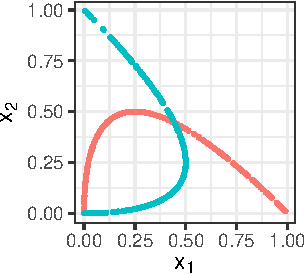
\includegraphics{draft_files/figure-latex/unnamed-chunk-2-1} 

}

\caption{Latent positions, labeled by curve/community.}\label{fig:unnamed-chunk-2}
\end{figure}

We draw $A \sim \mathrm{RDPG}(X)$ and obtain the following ASE:

\begin{figure}[H]

{\centering 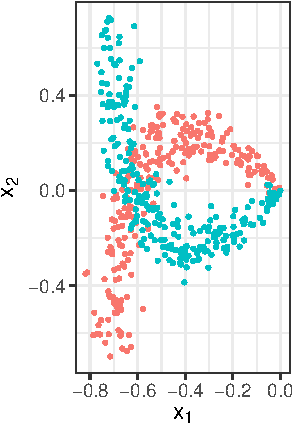
\includegraphics{draft_files/figure-latex/unnamed-chunk-3-1} 

}

\caption{ASE of an RDPG drawn from the latent positions, labeled by curve/community.}\label{fig:unnamed-chunk-3}
\end{figure}

We then try applying $K$-curves clustering to this graph. 
The first three are with random initial labels, forcing the intercept to be zero. 
The fourth initializes the labels randomly but allows the intercept to be nonzero. 
The fifth initializes the labels by spectral clustering with the normalized Laplacian, again forcing the intercept to be zero. 
The sixth also initializes via spectral clustering but allows the intercept to be nonzero. 



\begin{figure}[H]

{\centering 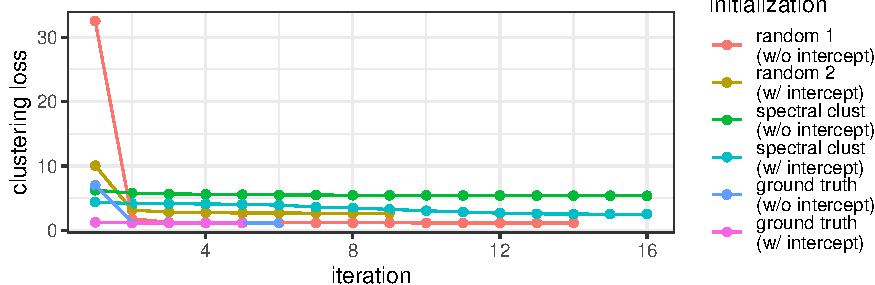
\includegraphics{draft_files/figure-latex/unnamed-chunk-5-1} 

}

\caption{Clustering loss vs. iteration for each run of K-curve clustering.}\label{fig:unnamed-chunk-5}
\end{figure}

\begin{figure}[H]

{\centering 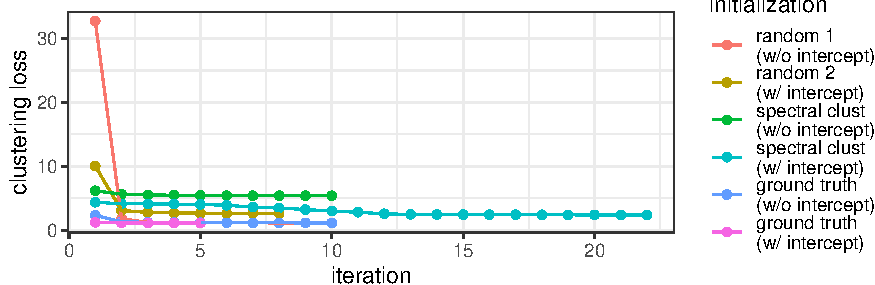
\includegraphics{draft_files/figure-latex/unnamed-chunk-6-1} 

}

\caption{ASE labeled by estimated community labels for each initialization strategy.}\label{fig:unnamed-chunk-6}
\end{figure}

\end{example}

\begin{example}[Macaque visuotactile brain areas and connections]


\begin{center}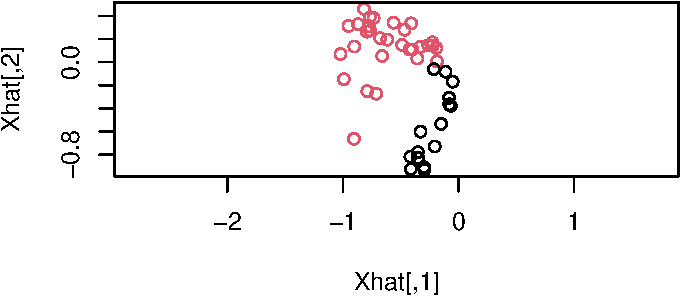
\includegraphics{draft_files/figure-latex/unnamed-chunk-7-1} \end{center}




\begin{center}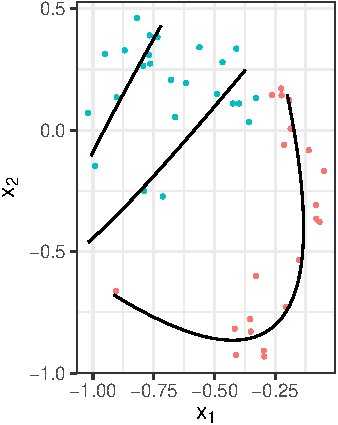
\includegraphics{draft_files/figure-latex/unnamed-chunk-9-1} \end{center}

\end{example}

\begin{example}[Non-intersecting curves]


\begin{center}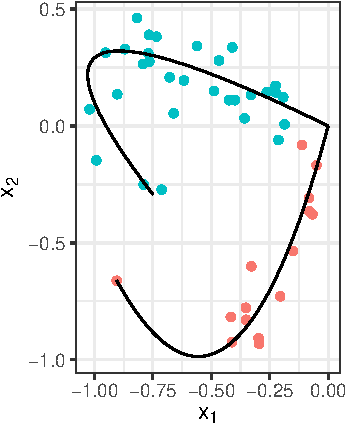
\includegraphics{draft_files/figure-latex/unnamed-chunk-10-1} \end{center}






\begin{center}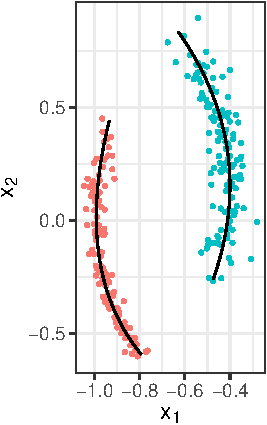
\includegraphics{draft_files/figure-latex/unnamed-chunk-13-1} \end{center}

\end{example}

\hypertarget{simulation-study}{%
\section{Simulation Study}\label{simulation-study}}

\bibliographystyle{agsm}
\bibliography{bibliography.bib}

\end{document}
